\documentclass[10pt,a4paper]{article}
\usepackage{polski}
\usepackage[utf8]{inputenc}
\usepackage{amsmath}
\usepackage{amsfonts}
\usepackage{amssymb}

\usepackage{inconsolata}
\renewcommand*\familydefault{\ttdefault} %% Only if the base font of the document is to be typewriter style
\usepackage[T1]{fontenc}


\usepackage{secdot}  % kropka po numerach sekcji
\usepackage{graphicx} % Required for the inclusion of images
\usepackage{geometry}
 \geometry{
 a4paper,
 total={170mm,257mm},
 left=25mm,
 right=25mm,
 top=20mm,
 }

% Kropki w spisie tresci
\usepackage[dotinlabels]{titletoc}
\titlecontents{chapter}
  [1.5em]
  {\addvspace{\baselineskip}}
  {\contentslabel{1.5em}\hspace*{0em}}
  {}
  {\titlerule*[1pc]{.}\contentspage}

%kod
\usepackage{listings}
\usepackage{color}
 
\definecolor{codegreen}{rgb}{0,0.6,0}
\definecolor{codegray}{rgb}{0.5,0.5,0.5}
\definecolor{codepurple}{rgb}{0.58,0,0.82}
\definecolor{backcolour}{rgb}{0.95,0.95,0.92}
 
\lstdefinestyle{mystyle}{
    backgroundcolor=\color{backcolour},   
    commentstyle=\color{codegreen},
    keywordstyle=\color{magenta},
    numberstyle=\tiny\color{codegray},
    stringstyle=\color{codepurple},
    basicstyle=\footnotesize,
    breakatwhitespace=false,         
    breaklines=true,                 
    captionpos=b,                    
    keepspaces=true,                 
    numbers=left,                    
    numbersep=5pt,                  
    showspaces=false,                
    showstringspaces=false,
    showtabs=false,                  
    tabsize=2,
    basicstyle=\normal    % rozmiar
}
 
\lstset{style=mystyle}
\renewcommand{\lstlistingname}{} %nazwa listingu
%
% instrukcjua jak z pliku to : \lstinputlisting[language=Ruby]{a.rb}
%
% jak nnormalnie to: \begin{lstlisting}[language=Ruby, caption=Ruby example]
%
% zdjecia:
% \begin{center}
%  \includegraphics[width=\textwidth]{nazwazdjeciabezrozszerzenia}
% \end{center}
%
% Kolory 
% \colorlet{Fuksjowy}{RubineRed!70!} i potem \textcolor{Fuksjowy}{Lorem ipsum...}
%
%
\usepackage[dvipsnames]{xcolor}
\definecolor{Mycolor2}{HTML}{FFFFED}
\pagecolor{Mycolor2}
\color{RoyalBlue}
%fuksjowy
\colorlet{Fuksjowy}{RubineRed!70!}

\title{Michał Bronikowski\protect\\ \hfill \protect\\ \protect\\ Systemy Operacyjne 2017 \protect\\ problem złodzieja jabłek \protect\\  {\small{wersja z procesami ciężkimi}} } % Title


\begin{document}
\maketitle  % Insert the title, author and date
\thispagestyle{empty}
\vfill
%© \scriptsize{Michał Bronikowski 2017}
\newpage
\tableofcontents
\newpage
\normalfont
\large
\section{Opis zadania}
\subsection{Problem złodzieja jabłek}
Problem został przeze mnie wymyślony na potrzeby zadania. Wzorowałem się na klasycznym problemie synchronizacji tj. problemie producenta i konsumenta.
Powiedzmy, że jesteśmy złodziejem jabłek i w naszej miejscowości są dwa sady A i B, w których w dość szybkim tempie przybywa jabłek. Kradniemy jabłka z
sadu A lub z sadu B. W międzyczasie w sadach, dzięki działaniu właścicieli i natury jabłek przybywa. Problem polega na takim zsynchronizowaniu procesów
sadów A i B oraz procesu złodzieja, żeby złodziej nie ukradł wszystkich jabłek z sadów, ponieważ to zwróciłoby uwagę właściciela i nasz złodziej mógłby mieć
problemy.
\subsection{Rozwiązanie}
W rozwiązaniu korzystam z dwóch semaforów:
\begin{itemize}
\item[•] skradziono
\item[•] uroslo
\end{itemize}
Złodziej czeka aż w sadach przybędzie jabłek co będzie skutkowało opuszczeniem semafara \textcolor{Fuksjowy}{uroslo}. Po czym przystępują do kradzieży jabłek z losowo wybranego przez siebie sadu. Po kradzieży zwalnia się semafor \textcolor{Fuksjowy}{skradziono}, a zamyka \textcolor{Fuksjowy}{uroslo}. Po zwolnieniu semafora \textcolor{Fuksjowy}{skradziono} w sadach ponownie rusza, produkcja jabłek.
\subsection{Implementacja}
Program należy uruchamiać na komputerze pod kontrolą systemu operacyjnego Linux. Program składa się z jednego pliku źródłowego sem.c. Załączony został również Makefile pomagający skompilować program.
\begin{lstlisting}[language=bash,caption=Skompilowanie programu poleceniem make]
  $ make
\end{lstlisting}
Program uruchamiamy poleceniem:
\begin{lstlisting}[language=bash,caption=Uruchomienie programu]
  $ ./sem
\end{lstlisting}
W programie zdefiniowałem strukturę \textcolor{Fuksjowy}{Zasob\_Dzielony}
\begin{lstlisting}[language=C,caption=struktura Zasob\_Dzielony]
struct Zasob_Dzielony
{
    sem_t skradziono ;
    sem_t uroslo ;
    int jablko_z_A ;
    int jablko_z_B ;
    int zA,zB;  
    int gdzie;
} *z_dz ;
\end{lstlisting}
Struktura zawiera elementy, które będą współdzielone przez wszystkie procesy programu.\\
Funkcja zarządzająca naszym złodziejem została zdefiniowana w następujący sposób:
\begin{lstlisting}[language=C,caption=Funkcja zarządzająca złodziejem,basicstyle=\footnotesize]
void zlodziej()
{   
    while(1)
    {
      sem_wait(&z_dz->uroslo);
      
      sad = rand()%2+1; 
      if(sad == 1)
      {
          if(z_dz->jablko_z_A < 1)
          {
              printf("Nie ukradne z sadu A - nie maja już jablek\n");
             
          } 
          else
          {
            --z_dz->jablko_z_A;
            z_dz->zA++;
          printf("Kradne jablko z sadu A mam juz %d jabłek z sadu A i %d jablek z sadu B \n ",z_dz->zA,z_dz->zB);
          }
          sem_post(&z_dz->skradziono);
          z_dz->gdzie=1;
      }
      else
      {   if(z_dz->jablko_z_B < 1)
          {
              printf("Nie ukradne z sadu B - nie maja juz jablek\n");
          }
          else
          {
          --z_dz->jablko_z_B;
          z_dz->zB++;
          printf("Kradne jablko z sadu B mam juz %d jabłek z sadu A i %d jablek z sadu B \n ",z_dz->zA,z_dz->zB);
          }
          sem_post(&z_dz->skradziono);
          z_dz->gdzie=2;
      }
         
    }
}
\end{lstlisting}
Po każdej dokonanej kradzieży złodziej zaznacza, z którego sadu ukradł jabłka, poprzez ustawienie wartości współdzielonej zmiennej \textcolor{Fuksjowy}{gdzie} odpowiednio na \textcolor{Fuksjowy}{1}
 lub \textcolor{Fuksjowy}{2}. Dzięki temu wiemy, w którym sadzie produkcja powinna ruszyć szybciej, aby w sad był konkurencyjny i nie zbankrutował (unikamy sytuacji, w której w sadzie nie będzie żadnego jabłka).\newpage Przejdźmy do zarządania sadami.
\begin{lstlisting}[language=C,caption=Funkcja zarządzająca produkcją jabłek w sadzie,basicstyle=\footnotesize]]
void rosnij()
{
    while (1)
    {
        sem_wait(&z_dz->skradziono);
        if((z_dz->gdzie) == 1)
        {
            printf("Jestem z sadu A i mam %d jablek\n", ++z_dz->jablko_z_A);
        }
        else
        {
            printf("Jestem z sadu  B i mam %d jablek\n", ++z_dz->jablko_z_B); 
        }
        sem_post(&z_dz->uroslo);
    }
}

\end{lstlisting}
Po zwolnieniu semafora \textcolor{Fuksjowy}{skradziono} sprawdzam, w którym sadzie ostatnio skradziono jabłka i tam przystępuję do produkcji kolejnych. W drugim sadzie jabłek nie powinno zostać, ponieważ reguluję wartość startową semaforów jako 5 zarówno dla złodzieja, jak i sadowników.\\ \\
W funkcji głównej programu inicjalizuję semafory i inicjalizuję wartości odpowiadające za ilość jabłek w poszczególnych sadach na 5.
\begin{lstlisting}[language=C,caption=Funkcja głowna,basicstyle=\footnotesize]]
int main()
{
    z_dz = mmap( NULL , sizeof( struct Zasob_Dzielony ) , PROT_READ | PROT_WRITE , MAP_SHARED | MAP_ANONYMOUS , -1 , 0 );
    sem_init( & z_dz->uroslo , 1 , 5 );
    sem_init( & z_dz->skradziono , 1 , 5 );
    z_dz->jablko_z_A = 5;
    z_dz->jablko_z_B = 5;
    pid = fork();
 
    if (pid < 0)
    {
        perror ("Niestety cos sie zepsulo :( \n");
        exit(1);
    } 
    else if (pid == 0)
    {
        rosnij();
        exit(0);
    }

    zlodziej();
    return 1;
}
\end{lstlisting}
Wartość zmiennej \textcolor{Fuksjowy}{pid} jest identyfikatorem procesu pid = 0 odpowiada za proces sadowników i pid = 1 określa proces złodzieja. Sprawdzam również, czy nie nastąpił niespodziewany błąd związany z uruchomionymi procesami, czyli przypadek, gdy pid < 0.
\section{Testowanie}
Chcąc sprawdzić, czy program rzeczywiście korzysta z procesów. Uruchamiamy go i jednocześnie sprawdzamy aktualnie działające procesy poleceniem:
\begin{lstlisting}[language=bash,caption=Polecenie wyświetlające działające procesy]
  $ ps -A
\end{lstlisting}
\begin{center}
  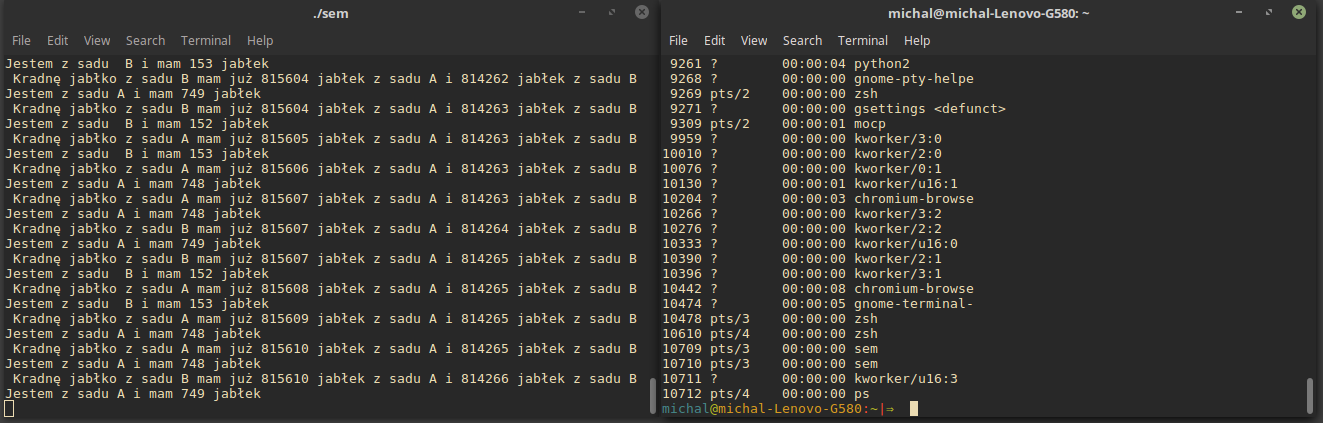
\includegraphics[width=\textwidth]{so1}
\end{center}
Procesy stworzone przez nasz program są widoczne jako:
\begin{center}
  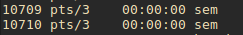
\includegraphics[]{so2}
\end{center}
\end{document}